% Chapter 5

\chapter{Motivations} % Chapter title

\label{ch:Motivations} % For referencing the chapter elsewhere, use \autoref{ch:name}

%----------------------------------------------------------------------------------------

\section{Radiative Corrections related issues}

In the past, COMPASS has been using two programs for radiative corrections estimation : one is TERAD, a program that
does analytic calculations of the (x,y)-dependant radiative correction factors, the other is RADGEN, which in addition
to the (x,y)-dependant radiative correction factors allows one to take into account a kinematic smearing caused by the
radiated photon. Despite being based on different QED calculation schemes, the two programs give compatible results for
both inclusive and semi-inclusive corrections in (x,y) kinematic domain.

Before going further in this discussion, some RADGEN formalism must be defined. The relations of the observed cross-section
$\sigma_{obs}$ with the 1-photon cross-section $\sigma_{1\gamma}$ are, for the inclusive case :

\begin{equation}
    \sigma_{obs} = (1+\delta_{vert}+\delta_{vac}+\delta_{sm})\sigma_{1\gamma}+\sigma_{el}+\sigma_{qel}+\sigma_{in}
\end{equation}

and for the semi-inclusive case :

\begin{equation}
    \sigma_{obs} = (1+\delta_{vert}+\delta_{vac}+\delta_{sm})\sigma_{1\gamma}+\sigma_{in}
\end{equation}

The difference between the two cases is only by $\sigma_{el}$ and $\sigma_{qel}$. The core of the problem is however in
the calculation of $\sigma_{in}$. The semi-inclusive radiative corrections are defined for the events with a hadron observed
in the final state. This fact is taken into account in $\sigma_{in}$ definition, viz. :

\begin{equation}
    \sigma_{in} = \int_{M+m_{\pi}}^{W}\sigma_{in}(M_{h},\theta_{max})dM_h
\end{equation}

The quantity $\sigma_{in}(M_{h},\theta_{max})$ is known and is not a problem but the lower limit of the integral is. In fact :

\begin{equation}
    W = M + M_{\pi}, E_{\gamma} = \frac{Q^2_{true}}{2M}+M_{\pi} \xrightarrow{Q^2_{true} \rightarrow 0} m_{\pi}
\end{equation}

As there must be energy conservation, a photon with $\nu = 1$ GeV interacting with a proton at rest cannot produce a hadron with
13 to 40 GeV. For hadrons observed in COMPASS, $\sigma_{in}$ will be smaller than results from TERAD or RADGEN.

When looking at the radiated photon energy distribution for HERMES kinematic ($x=0.1$, $y=0.8$, $E\approx27.5$ GeV, $\nu_{obs}\approx22$ GeV)
as represented in the lower-left panel of Fig. \ref{fig:RAD}, hard photon emissions are sizeable.

\begin{figure}[htb]
\centerline{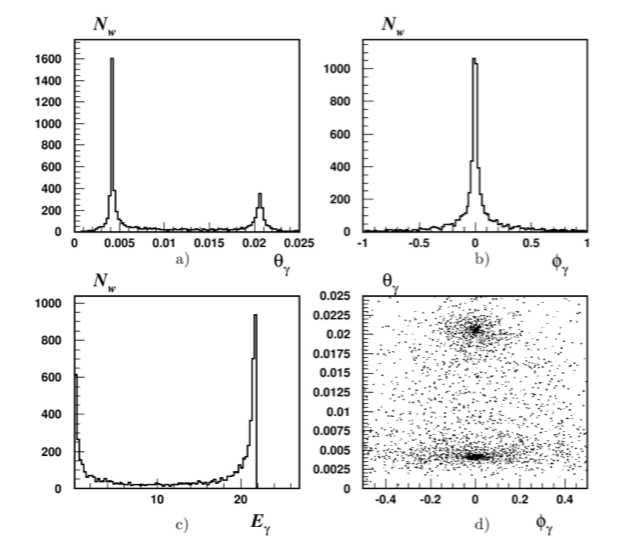
\epsfig{file=gfx/radgen.png,width=12cm}}
\caption{The distribution of the radiation angles $\theta_{\gamma}$ a), $\phi_{\gamma}$ b) and of the energy c) of the radiated
photon for $x=0.1$ and $y=0.8$. The two-dimensional distribution d) shows $\theta_{\gamma}$ vs $\phi_{\gamma}$. In panel c), one
can note that the hard photon emissions are sizeable.}\label{fig:RAD}
\end{figure}

Another point can be made by looking at actual COMPASS data, eg. 2006 data. As the $_{6}$LiD target has a non-negligible radiation length
part of photons will create $e^+e^-$ pairs and electrons from the conversion should be seen in the spectrometer. When performing Monte-Carlo generation
with COMGEANT+RADGEN, a large amount of electrons is produced. This can be brought into light by looking at the absolute value of the $\Phi$ angle
with respect to the lepton plane (see Fig. \ref{fig:elprod}).

\begin{figure}[htb!]
\centerline{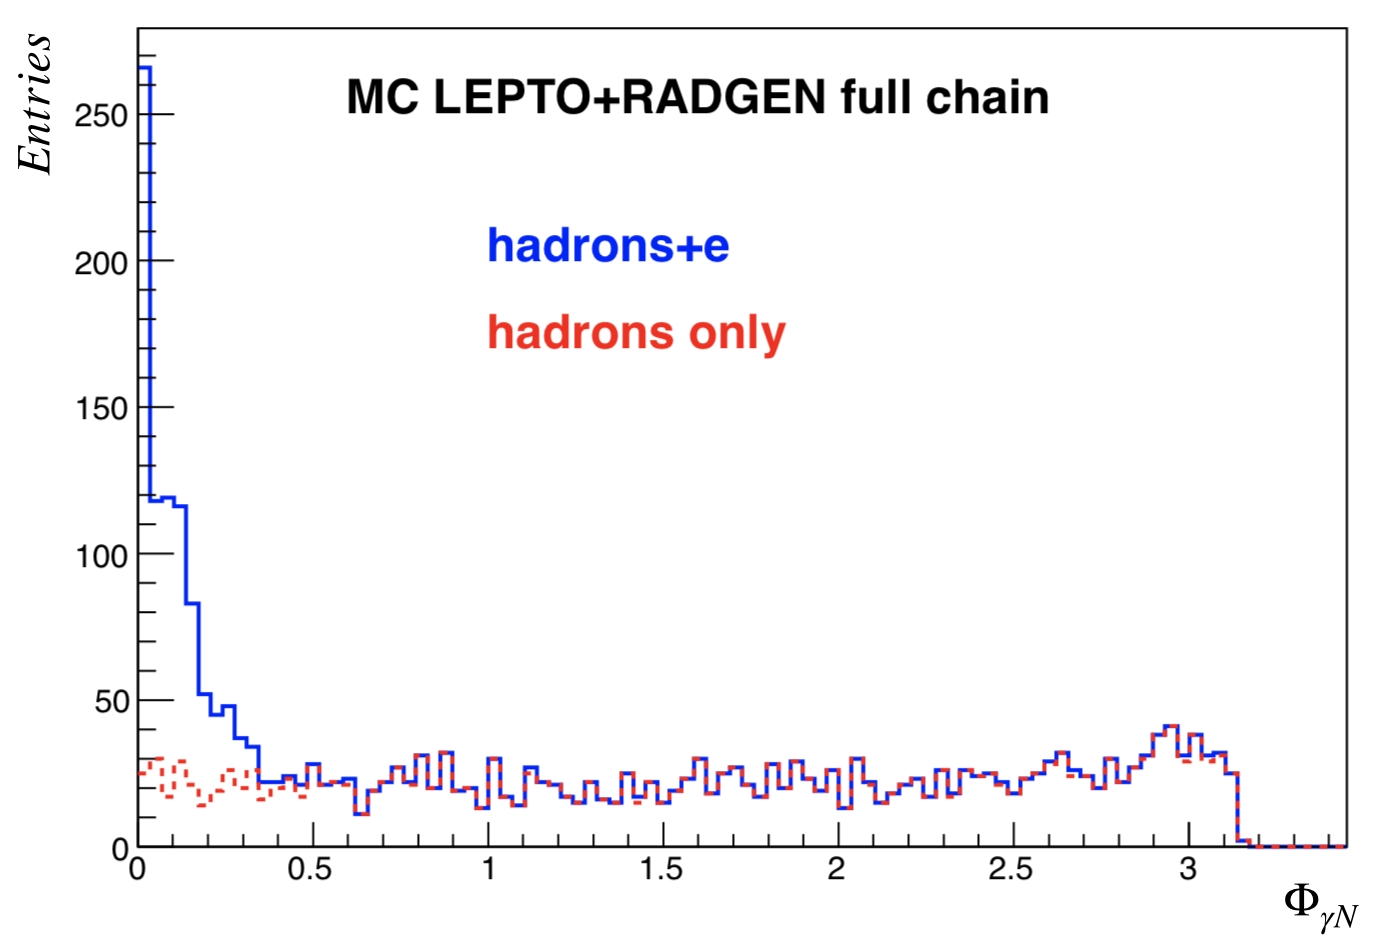
\epsfig{file=gfx/elprod.png,width=12cm}}
\caption{-}\label{fig:elprod}
\end{figure}

By comparing the Monte-Carlo generation with the real data for hadrons with $z>0.1$ and full $y$ range (Fig. \ref{fig:ph_pl}), one can note that on
average about 1.8 more electrons are produced in Monte-Carlo than in real data.

\begin{figure}[htb!]
\centerline{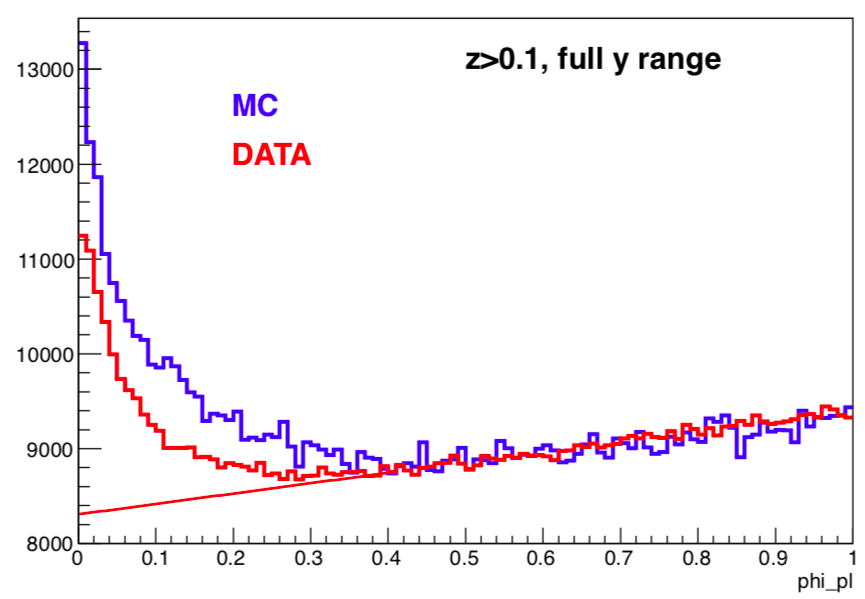
\epsfig{file=gfx/ph_pl.png,width=12cm}}
\caption{-}\label{fig:ph_pl}
\end{figure}

%----------------------------------------------------------------------------------------

\section{Comparison between RADGEN and DJANGOH}

As one saw in the previous section, a rather problematic result is happening with RADGEN : the generator is
producing a high number of hard photons leading to great discrepancies with the real data. The comparison between
DJANGOH, which will be presented in the next chapter, and RADGEN can inform us on the possible better description
of our data by DJANGOH if the generator is producing way less hard photons than RADGEN. In Fig. \ref{fig:DJRAD},
the $E_{\gamma}$ is compared and one can already see that overall, without comparing any number, DJANGOH is producing
less hard photons than soft photons when this is the complete inverse for RADGEN.

\begin{figure}[htb]
\centerline{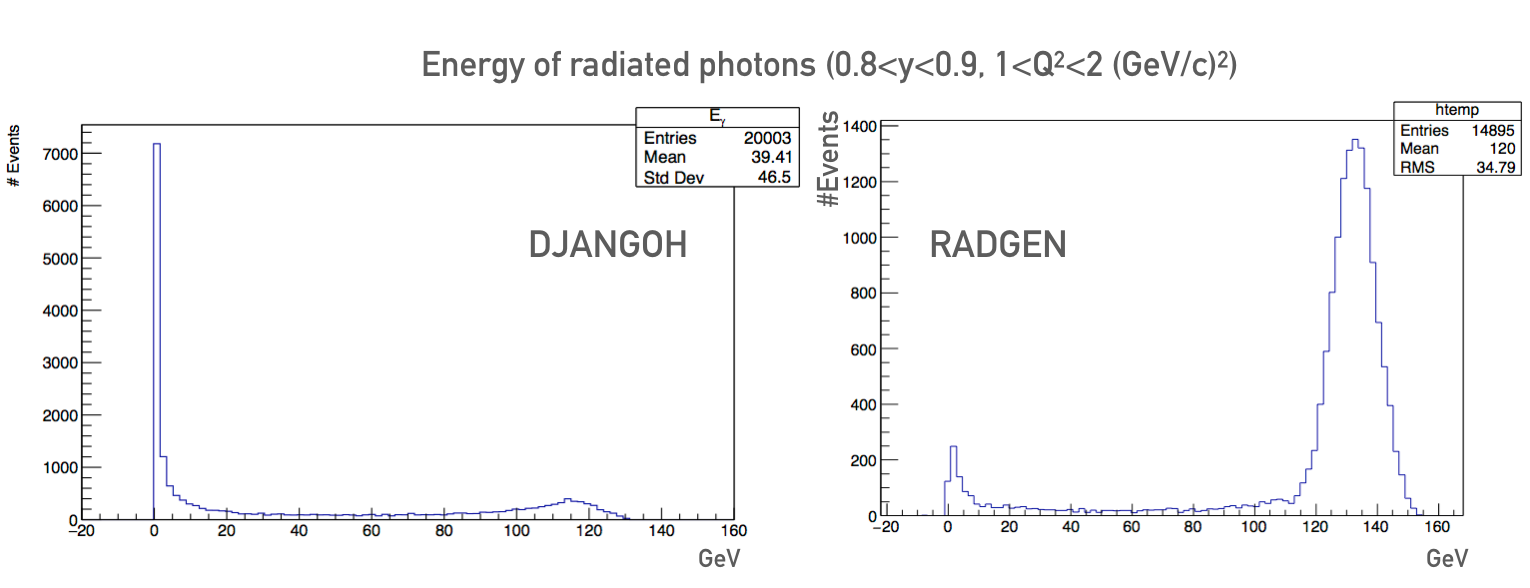
\epsfig{file=gfx/DJRAD.png,width=12cm}}
\caption{Left is the radiative photon energy distribution for $0.8 \leq y \leq 0.9$ and $1 \leq Q^2 \leq 2 (GeV/c)^2$ for DJANGOH, right is the same distribution for RADGEN.
DJANGOH is producing overall more soft photons than hard ones, unlike RADGEN. Nevertheless, the plot does not allow
to conclude whether DJANGOH is producing less hard photon than RADGEN.}\label{fig:DJRAD}
\end{figure}

By comparing more thoroughly, computing the proportion of inelastic events in the range between 20 and 160 GeV
over the total number of DIS events (Fig. \ref{fig:tabDJRAD}), RADGEN has a total of 18.6\% of event in this
area when DJANGOH reaches a total of only 8.6\%. We can then definitely claim that DJANGOH is producing less
hard photons than RADGEN, which is encouraging for the comparison to real data.

\begin{figure}[htb]
\centerline{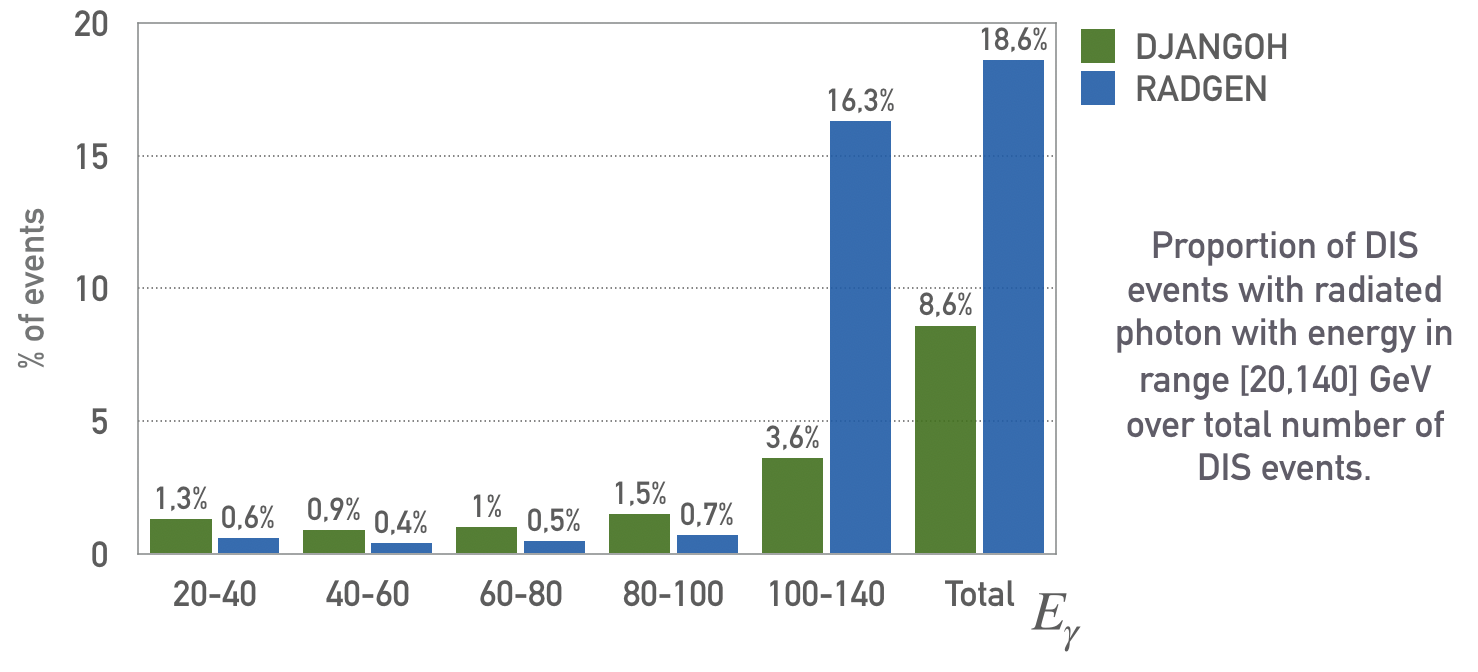
\epsfig{file=gfx/tabDJRAD.png,width=12cm}}
\caption{Comparison of proportion of inelastic event in high energy radiative photon range over total number
of DIS event with the same kinematical restrictions as in Fig. \ref{fig:DJRAD}. This comparison allows to conclude that DJANGOH is indeed producing less hard photons than
RADGEN with more than a factor 2 between the two generators. Thus, RADGEN is producing much less
soft photons than DJANGOH, when referring to Fig. \ref{fig:DJRAD} with this knowledge.}\label{fig:tabDJRAD}
\end{figure}
